\documentclass{standalone}

\usepackage{tikz,tikz-3dplot,pgfplots,xcolor}
\usetikzlibrary{arrows.meta,calc}
\usetikzlibrary{decorations.markings}

\usepackage{amsmath}

\newcommand{\derivative}[2]{\frac{\partial #1}{\partial #2}}
\newcommand{\dderivative}[2]{\frac{\partial^2 #1}{\partial {#2}^2}}
\renewcommand{\exp}[1]{\ {\rm exp}\left( {#1} \right)}
\newcommand{\ext}[1]{#1^{\rm ext}}
\newcommand{\red}[1]{#1_{\rm red}}
\newcommand{\redn}[1]{#1_{\rm red,n}}
\newcommand{\inve}[1]{#1^{e-1}}
\newcommand{\transpose}[1]{#1^{\top}}
\newcommand{\ue}[1]{\underline{#1}^{e}}
\newcommand{\eT}[1]{{#1}^{e \top}}
\newcommand{\uT}[1]{\underline{#1}^{\top}}
\newcommand{\uprime}[1]{\underline{#1}^{\prime}}
\newcommand{\uTprime}[1]{\underline{#1}^{\prime \top}}
\newcommand{\vect}[1]{{\bf{#1}}}
\renewcommand{\sin}[1]{\ {\rm sin}\left( {#1} \right)}
\renewcommand{\sinh}[1]{\ {\rm sinh}\left( {#1} \right)}
\renewcommand{\cos}[1]{\ {\rm cos}\left( {#1} \right)}
\renewcommand{\cosh}[1]{\ {\rm cosh}\left( {#1} \right)}


\newcommand{\BB}{\vect{B}}
\newcommand{\BBT}{\transpose{\vect{B}}}
\newcommand{\BBe}{\vect{B}^e}
\newcommand{\BBeT}{\eT{\vect{B}}}

\newcommand{\cc}{\vect{c}}
\newcommand{\CC}{\vect{C}}
\newcommand{\cce}{\vect{c}^e}
\newcommand{\CCe}{\vect{C}^e}
\newcommand{\CCei}{\vect{C}^e_i}
\newcommand{\ccek}{\vect{c}^e_{\rm k}}
\newcommand{\ccen}{\vect{c}^e_{\rm n}}
\newcommand{\ccenI}{\vect{c}^e_{\rm n+1}}
\newcommand{\cck}{\cc_{\rm k}}
\newcommand{\ccn}{\vect{c}_{\rm n}}
\newcommand{\ccnred}{\redn{\cc}}
\newcommand{\ccred}{\red{\cc}}
\newcommand{\CCred}{\red{\CC}}

\newcommand{\cdt}{\dot{c}}
\newcommand{\cdtue}{\ue{\dot{c}}}
\newcommand{\cie}{c_i^e}
\newcommand{\cprime}{c^{\prime}}
\newcommand{\cpprime}{c^{\prime \prime}}
\newcommand{\cu}{\underline{c}}
\newcommand{\cue}{\ue{c}}
\newcommand{\cceT}{\eT{c}}
\renewcommand{\rmd}{{\rm d}}

\newcommand{\FF}{\vect{F}}
\newcommand{\FFe}{\vect{F}^e}
\newcommand{\FFext}{\ext{\FF}}
\newcommand{\FFred}{\red{\FF}}

\newcommand{\jje}{\vect{j}^e}
\newcommand{\Je}{J^{e}}
\newcommand{\Jeinv}{\inve{J}}
\newcommand{\jprime}{j^{\prime}}

\newcommand{\KK}{\vect{K}}
\newcommand{\KKe}{\vect{K}^e}
\newcommand{\KKei}{\vect{K}^e_i}
\newcommand{\KKred}{\red{\KK}}

\newcommand{\LLe}{\vect{L}^{e}}
\newcommand{\LLeT}{\eT{\vect{L}}}
\newcommand{\Nel}{N_{\rm el}}
\newcommand{\Nen}{N_{\rm en}}
\newcommand{\Nie}{N_i^e}
\newcommand{\Nip}{N_{\rm ip}}
\newcommand{\NN}{\vect{N}}
\newcommand{\NNe}{\vect{N}^e}
\newcommand{\NNeT}{\eT{\vect{N}}}
\newcommand{\NNT}{\transpose{\vect{N}}}
\newcommand{\Omegae}{\Omega^{e}}
\newcommand{\vv}{\vect{v}}
\newcommand{\vvT}{\transpose{\vect{v}}}
\newcommand{\vve}{\vect{v}^e}
\newcommand{\vveT}{\eT{\vect{v}}}
\newcommand{\xxe}{\vect{x}^e}

\newcommand{\zzero}{\vect{0}}


\newcommand{\dx}{\rmd x}
\newcommand{\dxi}{\rmd \xi}
\newcommand{\dxDxi}{\derivative{x}{\xi}}
\newcommand{\dDt}{\frac{\partial}{\partial t}}
\newcommand{\Dt}{\Delta t}
\newcommand{\dcDx}{\derivative{c}{x}}
\newcommand{\dcDxi}{\derivative{c}{\xi}}
\newcommand{\dcDt}{\derivative{c}{t}}
\newcommand{\dccDt}{\derivative{\cc}{t}}
\newcommand{\dcceDt}{\derivative{\cce}{t}}
\newcommand{\ddcDDx}{\dderivative{c}{x}}
\newcommand{\djDx}{\derivative{j}{x}}
\newcommand{\dGDt}{\derivative{G}{t}}
\newcommand{\dphiDx}{\derivative{\varphi}{x}}
\newcommand{\ddphiDDx}{\dderivative{\varphi}{x}}
\newcommand{\dNieDx}{\derivative{\Nie}{x}}
\newcommand{\dvDx}{\derivative{v}{x}}
\newcommand{\ddvDDx}{\dderivative{v}{x}}
\newcommand{\dvDt}{\derivative{v}{t}}

\newcommand{\intl}{\int\displaylimits_{x=0}^{l}}
\newcommand{\intOmega}{\int\displaylimits_{\Omega}}
\newcommand{\intOmegae}{\int\displaylimits_{\Omegae}}
\newcommand{\intXi}{\int\displaylimits_{\xi=-1}^{1}}
\newcommand{\sumel}{\sum_{e=1}^{\Nel}}
\newcommand{\sumip}{\sum_{i=1}^{\Nip}}
\newcommand{\sumNen}{\sum_{i=1}^{\Nen}}



%\pgfplotsset{compat=1.18} 
\definecolor{blue1}{rgb}{0.88,0.88,0.98}
\definecolor{blue2}{rgb}{0.18,0.18,0.78}
\definecolor{blue3}{rgb}{0.28,0.28,0.68}
\definecolor{gray0}{rgb}{0.98,0.98,0.98}
\definecolor{gray1}{rgb}{0.8,0.8,0.8}
\definecolor{gray2}{rgb}{0.7,0.7,0.7}
\definecolor{gray3}{rgb}{0.6,0.6,0.6}
\definecolor{gray4}{rgb}{0.4,0.4,0.4}
\definecolor{gray5}{rgb}{0.25,0.25,0.25}
\definecolor{gray6}{rgb}{0.1,0.1,0.1}

\begin{document}

  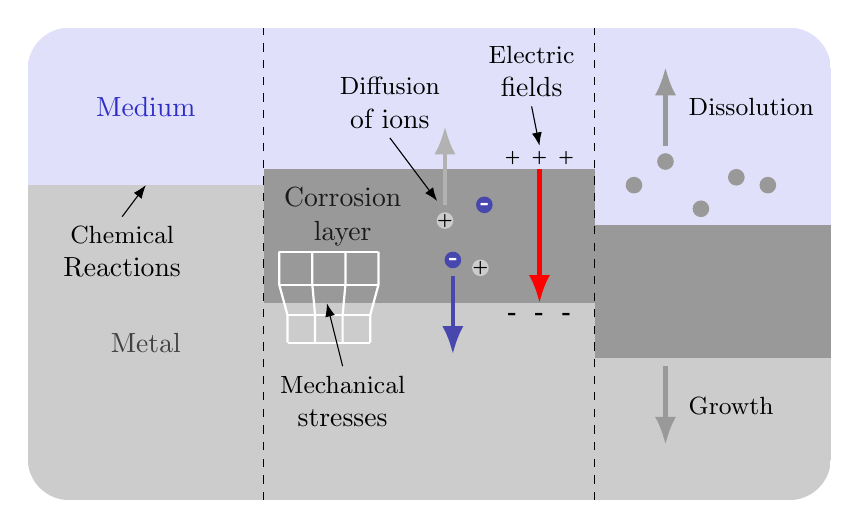
\begin{tikzpicture}[>=Latex
    ]
    \clip[rounded corners=15pt] (0,0) rectangle (10.2,6);
    \path[fill=gray1] (0,0) rectangle ++(3,4);
    \path[fill=blue1] (0,4) rectangle ++(3,2);
    \path[fill=gray1] (3,0) rectangle ++(4.2,4);
    \path[fill=blue1] (3,4) rectangle ++(4.2,2);
    \path[fill=gray3] (3,2.5) rectangle ++(4.2,1.7);
    \path[fill=gray1] (7.2,0) rectangle ++(3,1.8);
    \path[fill=gray3] (7.2,1.8) rectangle ++(3,1.7);
    \path[fill=blue1] (7.2,3.5) rectangle ++(3,2.5);
    \draw[dashed](3,0)--++(0,6);
    \draw[dashed](7.2,0)--++(0,6);
    \draw[<-] (1.5,4) --++ (-0.3,-0.4) node[below,align=center]{\small Chemical\\Reactions};
    \node[gray5] at (1.5,2){Metal};
    \node[blue2] at (1.5,5){Medium};
    \node[gray6,align=center] at (4,3.6){Corrosion\\layer};


    \begin{scope}[shift={(5.8,3.75)}]
      \path[fill,blue3] (0,0) circle (3pt) node[white,shift={(0.2pt,0.1pt)}]{\bf\footnotesize -};
      \path[fill,gray1] (-0.5,-0.2) coordinate(co1) circle (3pt) node[black]{\bf \tiny +};
      \path[fill,blue3] (-0.4,-0.7) coordinate(co2) circle (3pt) node[white,shift={(0.2pt,0.1pt)}]{\bf\footnotesize -};
      \path[fill,gray1] (-0.05,-0.8) circle (3pt) node[black]{\bf \tiny +}; 
      \draw[ultra thick,->,gray2] ($(co1)+(0,0.2)$)--++(0,1);
      \draw[ultra thick,->,blue3] ($(co2)+(0,-0.2)$)--++(0,-1);
    \end{scope} 

    \begin{scope}[shift={(3.3,2)},scale=0.7]
      \draw[white,thick] (0,0) --++ (1.5,0);
      \draw[white,thick] (0,0.5) --++ (1.5,0);
      \draw[white,thick] (-0.15,1.05) --++ (1.8,0);
      \draw[white,thick] (-0.15,1.65) --++ (1.8,0);
      \draw[white,thick] (0,0) -- (0,0.5) -- (-0.15,1.05)--(-0.15,1.65);
      \draw[white,thick] (0.5,0) -- (0.5,0.5)--(0.45,1.05)--(0.45,1.65);
      \draw[white,thick] (1,0) -- (1,0.5)--(1.05,1.05)--(1.05,1.65);
      \draw[white,thick] (1.5,0) -- (1.5,0.5)--(1.65,1.05)--(1.65,1.65);
    \end{scope}

    \draw[<-] (3.8,2.5)--++(0.2,-0.8) node[align=center,below]{\small Mechanical\\stresses}; 
    \draw[<-] (5.2,3.8)--++(-0.6,0.8) node[align=center,above]{\small Diffusion \\ of ions};
    \draw[<-] (6.5,4.5)--++(-0.1,0.5) node[align=center,above]{\small Electric \\ fields};
    \draw[->,red,ultra thick] (6.5,4.2) --++(0,-1.7) node[right,pos=0.5,black]{$\EE$}; 
    \node at (6.5,4.35){\tiny \bf +\, + \,+};
    \node at (6.5,2.35){\footnotesize \bf - \ - \ -};

    \begin{scope}[shift={(8.6,4.5)}]
      \path[fill,gray3] (0.8,-0.5) circle (3pt);
      \path[fill,gray3] (-0.5,-0.2) coordinate(co1) circle (3pt);
      \path[fill,gray3] (0.4,-0.4)  circle (3pt);
      \path[fill,gray3] (-0.05,-0.8) circle (3pt); 
      \path[fill,gray3] (-0.9,-0.5) circle (3pt); 
      \draw[ultra thick,->,gray3] ($(co1)+(0,0.2)$)--++(0,1)node[right=0.15cm,black,align=center,pos=0.5]{\small Dissolution};
      \draw[ultra thick,->,gray3] ($(co1)+(0,-2.6)$)--++(0,-1) node[right=0.15cm,black,align=center,pos=0.5]{\small Growth};
    \end{scope} 
   

  \end{tikzpicture}
\end{document} 